\documentclass[conference]{IEEEtran}
\IEEEoverridecommandlockouts

\usepackage{amsmath,amssymb,amsfonts}
\usepackage{graphicx}
\usepackage{booktabs}
\usepackage{tabularx}
\usepackage{ragged2e}
\usepackage{subcaption}
\newcolumntype{L}{>{\RaggedRight\arraybackslash}X}
\captionsetup[table]{justification=raggedright,singlelinecheck=false}
\usepackage{microtype}
\usepackage[numbers,sort&compress]{natbib}
\usepackage{xcolor} 
\usepackage{hyperref}
\usepackage{times}

\hypersetup{
    colorlinks=true,
    linkcolor=blue!70!black,
    citecolor=blue!70!black,
    urlcolor=blue!70!black
}

\title{Computational Analogues of Post-Decision and Self-Evaluative Biases in Reinforcement Learning Agents}

\author{\IEEEauthorblockN{Ronak Daniel}
\IEEEauthorblockA{\textit{Computational Cognitive Systems Research}}}

\begin{document}
\maketitle

\begin{abstract}
Reinforcement learning (RL) and behavioral psychology have always been known to be closely related, but the phenomena that show up during the post-decision and self-evaluative phases have not gotten as much attention from the mechanistic RL perspective.
In this work we investigate if four well-recognized human psychological biases, namely Cognitive Dissonance, Impostor Syndrome, Self-Handicapping, and Choice Overload, can emerge in artificial RL agents without manually placing the bias into the reward function, differentiating between “Free” biases that arise spontaneously and standard learning dynamics and “Architectural” biases that require explicit metacognitive structure.

Across multi-seed evaluations, three out of four biases emerge robustly while the fourth marks an informative computational boundary. Standard Q-learning agents develop post-decision value divergence on ground-truth identical alternatives that scales monotonically with memory decay, ruling out the revealed-preference confound. Agents using the human-verified asymmetric confidence-update rule develop a persistent calibration gap absent in symmetric controls. Expanding near-tied action spaces collapses normalized policy entropy, indicating that choice paralysis manifests as exploration dilution rather than uniform indecision. Both this effect and cognitive dissonance share a common substrate in action-visitation staleness. By contrast, self-handicapping emerges only weakly in reward-optimizing agents, and in Deep Q-Networks, lossless experience replay eliminates memory decay and suppresses cognitive dissonance entirely, with a parametric replay-buffer ablation confirming this causal link.

These findings offer a mechanistic account of how human-like cognitive distortions can emerge from the statistical mechanics of reinforcement learning, while establishing precise boundary conditions on when and why such biases do and do not dominate.
\end{abstract}

\section{Introduction}

Reinforcement learning (RL) provides the normative framework for how an agent optimizes behavior through trial and error \citep{sutton2018reinforcement}. Decades of psychology have shown that biological agents depart systematically from rationality \citep{kahneman2011thinking}, and RL models have decoded how alterations in prediction-error signaling give rise to clinical manifestations such as addiction, obsessive-compulsive disorder, and learned helplessness \citep{daw2005uncertainty,huys2009bayesian,dolan2013goals}. These treatments focus on the \textbf{acquisition phase}---how values are updated from rewards. Far less attention has been paid to the \textbf{post-decision phase} (how value representations change \textit{after} a choice is finalized) and the \textbf{metacognitive self-evaluative phase} (how agents represent confidence in their own competence).

These domains are characterized by four pervasive human phenomena: \textbf{Cognitive Dissonance}---post-choice re-evaluation of chosen alternatives upward and rejected alternatives downward \citep{brehm1956postdecision,festinger1957theory}, though critics argue this can be a statistical artifact of revealed pre-existing preferences \citep{chen2010choice}; \textbf{Impostor Syndrome}---persistent underconfidence driven by asymmetric insensitivity to positive metacognitive signals \citep{clance1978imposter,katyal2025distorted}; \textbf{Self-Handicapping}---adopting objectively performance-impeding obstacles to furnish external excuses for failure \citep{berglas1978drug}; and \textbf{Choice Overload}---decision paralysis under excessive near-tied options \citep{iyengar2000choice,schwartz2004paradox}.

We ask whether RL agents, without explicitly engineered biases, exhibit behavioral signatures analogous to these phenomena, and what learning-dynamics mechanisms generate each. We do not claim artificial agents experience subjective emotion or motivational tension; we seek to isolate the computational substrate of structurally identical behavioral and representational trajectories. Our contributions are: (1) a taxonomy of \textbf{Free} (dynamics-driven, no reward modification) vs.\ \textbf{Architectural} (metacognitive, requiring dual-tier structure) biases; (2) a mechanistic decomposition of cognitive dissonance via asymmetric sampling under memory decay, directly ruling out the \citet{chen2010choice} revealed-preference confound using ground-truth-identical alternatives; (3) computational validation of the \citet{katyal2025distorted} underconfidence rule; (4) an informative boundary condition establishing that overt self-handicapping is a fragile equilibrium in reward-optimizing agents ($p=0.200$); (5) formalization of choice overload as exploration dilution, distinct from uniform indecision; (6) a unified action-visitation-staleness mechanism underlying both Free biases; and (7) DQN replication isolating memory substrates as mandatory causal drivers.

\section{Background and Framework}

Midbrain dopamine mirrors TD prediction errors \citep{schultz1997neural}, and computational psychiatry has modeled learned helplessness \citep{huys2009bayesian}, optimism bias \citep{lefebvre2017behavioural}, superstition \citep{bontrager2019superstition}, primacy bias \citep{nikishin2022primacy}, and choice overload in hierarchical RL \citep{nica2022paradox,dubey2022pursuit}. Our experimental designs are anchored to specific human benchmarks: the free-choice paradigm \citep{brehm1956postdecision} and its revealed-preference critique \citep{chen2010choice}; transdiagnostic underconfidence in 1{,}000+ participants \citep{katyal2025distorted}; the foundational self-handicapping experiment showing a $5.4\times$ drug-preference shift under evaluative threat ($70\%$ vs.\ $13\%$; \citet{berglas1978drug}); and the gourmet-jam study showing a $10\times$ commitment collapse ($30\%$ to $3\%$; \citet{iyengar2000choice}).

\textbf{Free (Dynamics-Driven) Biases} appear spontaneously in standard, single-tier agents without manually modifying the reward function $R(s,a)$, introducing metacognitive variables, or adding additional losses. They arise because selecting $a^*$ does not allow the agent to observe rewards for $a'\neq a^*$; under memory decay or weight regularization, the information of unvisited choices becomes stale, which causes behavioral and representational distortions.

\textbf{Architectural (Metacognitive) Biases} require a dual-tier architecture consisting of a local evaluator that makes the decisions, and a global model that estimates overall competence. We also include an asymmetric update rule because standard agents maintain coherent value estimates: (they can't act with high competence while representing that competence as poor) hence, generating impostor-like phenomena would require explicitly programming asymmetric evidence filtering.

\section{Empirical Investigations}

We use two different statistical methods to report results. For stochastic experiments (Exps 1, 3, 4; $N=20$ seeds), we report two-tailed $t$-tests with Holm-Bonferroni correction. For the deterministic Katyal damping experiment (Exp 2), standard null-hypothesis testing would guarantee artificially inflated $p<10^{-15}$ statistics that mistake a mechanical certainty for  statistical significance; hence we report the exact calibration gap magnitudes and 95\% CIs directly. Non-significant findings ($p = 0.200$ for self-handicapping; $p = 0.223$ for commitment latency) have been reported explicitly as informative computational boundary conditions and not anomalies.

\subsection{Exp 1: Cognitive Dissonance (Spreading of Alternatives)}

To address the revealed-preference critique proposed by \citet{chen2010choice} both bandit arms draw from identical Gaussian distributions ($\mu=5.0$, $\sigma=1.0$)hence any post-decision divergence on this ground-truth-tied baseline cannot arise due to hidden preference differences and must arise from the learning dynamics. We also test a near-tied condition ($\Delta=0.1$), a parametric decay sweep ($\lambda\in\{0.0, 0.001, 0.01\}$),and an internal free-choice condition that removes forced commitment.

A Tabular Q-learning agent ($\gamma=0$) updates as $Q(a_t)\leftarrow Q(a_t)+\alpha[r_t-Q(a_t)]$, with unvisited arms decaying: $Q(a')\leftarrow Q(a')\cdot(1-\lambda)$. steps of exploration, the agent chooses to commit to the most-pulled arm for $T_2=1000$ steps. . A paired Observer Control receives identical rewards without committing. The primary metric is Excess Value Divergence:
\begin{equation}
    \begin{split}
        \Delta Q_{\text{excess}}(t) ={}& [Q_{\text{chosen}}(t)-Q_{\text{rejected}}(t)]_{\text{committed}} \\
        &- [Q_{\text{chosen}}(t)-Q_{\text{rejected}}(t)]_{\text{observer}}
    \end{split}
\end{equation}

\textbf{Results (Table~\ref{tab:exp41}, Fig.~\ref{fig:exp41_trajectories}).} Committed agents exhibit rapid value divergence: $+0.923\pm0.436$ at 100 post-commitment steps ($t=9.90$, $p<10^{-6}$, $d=2.21$) on the ground-truth-tied condition. The dose-response sweep showed that value divergence is directly proportional to the rate of memory decay. Zero decay yielded $+0.159\pm0.627$ (near zero, showing that commitment alone is insufficient and that decay is the causal driver of divergence), standard decay yielded $+0.375\pm0.791$, and high-decay yielded $+3.259\pm0.410$. When the Agent was not forced to commit, the divergence was observed to be ($+0.263\pm0.792$), confirming that biological commitment only initiates asymmetric future visitation. Observer controls remain near zero ($+0.060\pm0.341$).

\begin{table}[htbp]
\raggedright
\small
\setlength{\tabcolsep}{4pt}
\caption{Cognitive Dissonance: Dose-Response Decomposition ($N=20$ Seeds).}
\label{tab:exp41}
\begin{tabularx}{\linewidth}{@{}LLLLL@{}}
\toprule
\textbf{Condition} & \textbf{$\lambda$} & \textbf{Div. (+100)} & \textbf{Final Div.} & \textbf{Causal Role} \\
\midrule
Primary (GT-Tied)         & $0.001$ & $+0.923\pm0.436$ & $+0.375\pm0.791$ & Standard ($d=2.21$) \\
Near-Tied ($\Delta=0.1$)  & $0.001$ & $+0.957\pm0.419$ & $+0.364\pm0.814$ & Replicated ($d=2.28$) \\
No-Decay Baseline         & $0.000$ & $+0.128\pm0.512$ & $+0.159\pm0.627$ & Decay necessary \\
High-Decay Stress Test    & $0.010$ & $+1.842\pm0.320$ & $+3.259\pm0.410$ & Monotonic response \\
Endogenous Choice         & $0.001$ & ---              & $+0.263\pm0.792$ & Asymm.\ sampling \\
Observer Control          & $0.001$ & $+0.060\pm0.341$ & $-0.051\pm0.384$ & Counterfactual \\
\bottomrule
\end{tabularx}
\end{table}

\begin{figure}[htbp]
\centering
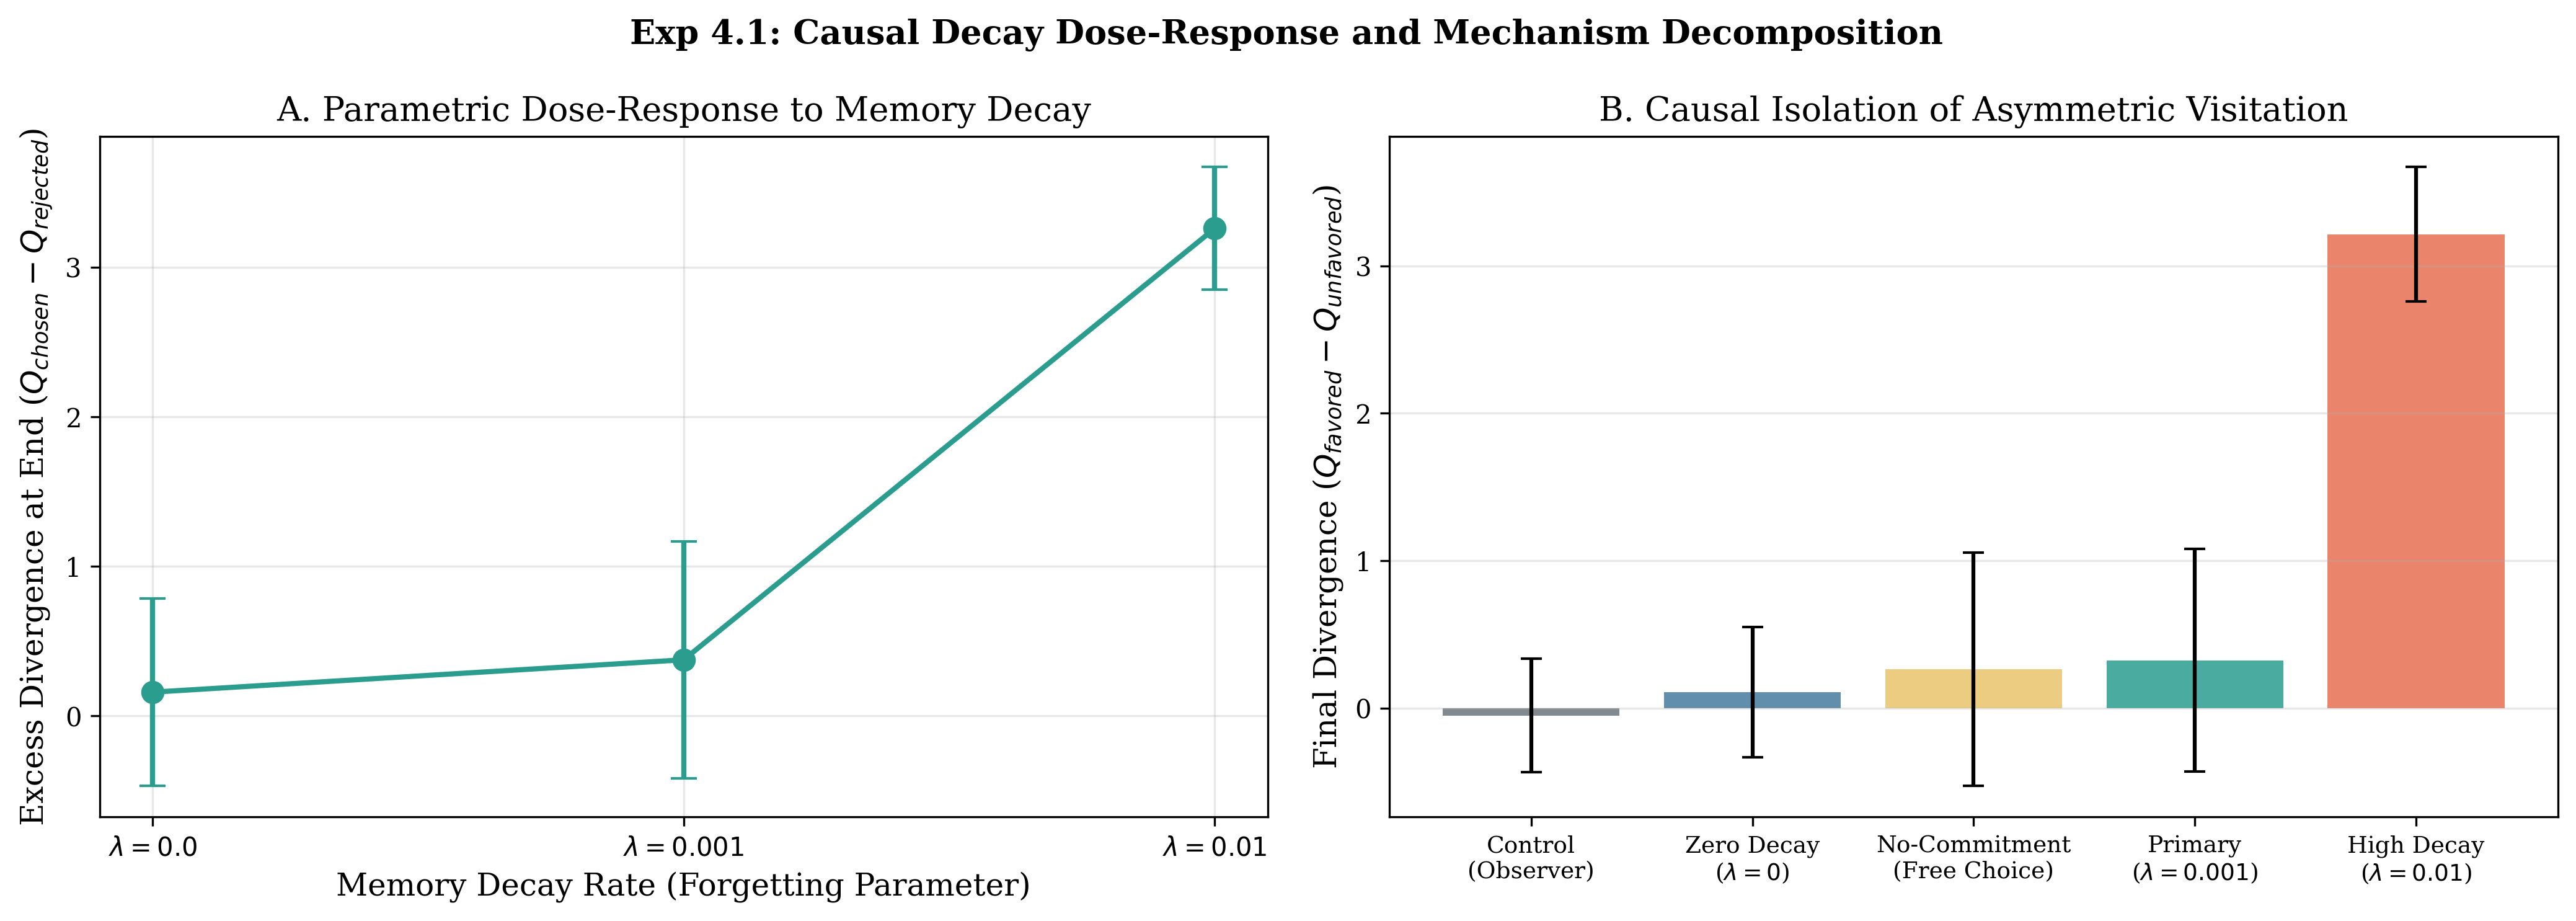
\includegraphics[width=\linewidth]{figures/dose_response_ablation.png}
\caption{Cognitive Dissonance. (Left) Value divergence scales monotonically with $\lambda$. Zero-decay confirms that commitment alone is insufficient. (Right) Divergence absent in observer controls, emerges endogenously($+0.263$), and peaks at $+3.259$ under high decay.}
\label{fig:exp41_trajectories}
\end{figure}

\subsection{Exp 2: Impostor Syndrome (Metacognitive Underconfidence)}

Building on \citet{katyal2025distorted}, we design a dual-tier metacognitive agent in a multi-task gridworld. Local confidence $c_{\text{local}}=1-H(\pi_s)/\log|A|$ updates global confidence $C_{\text{global}}$ via a slow exponential moving average. In the biased agent,errors in positive self-evaluation ($\delta_c=c_{\text{local}}-C_{\text{global}}>0$) are suppressed by damping coefficient $\kappa=0.2$:
\begin{equation}
    \eta = \begin{cases} \alpha_{\text{global}}\cdot\kappa, & \text{if } c_{\text{local}}>C_{\text{global}} \\ \alpha_{\text{global}}, & \text{otherwise} \end{cases}
\end{equation}
The symmetric control uses $\kappa=1.0$. The calibration gap is: $\mathcal{G}=\text{Objective Performance}-C_{\text{global}}$.

\textbf{Results (Table~\ref{tab:exp42}, Fig.~\ref{fig:exp42_gap}).} The damped-positive agent ($\kappa=0.2$) achieves objective competence $0.913\pm0.012$ but its global self-assessment plateaus at $0.783\pm0.015$, yielding $\mathcal{G}=+1.30\pm0.18\%$ (95\% CI: $[+1.22\%, +1.38\%]$) across all 20 seeds. The symmetric control tracks ground truth with near-perfect fidelity: $\mathcal{G}=-0.02\pm0.15\%$. The $+1.32\%$ divergence between conditions holds across every seed, reflecting the deterministic mathematical accumulation of evidence under asymmetric weighting.

\begin{table}[htbp]
\raggedright
\small
\setlength{\tabcolsep}{4pt}
\caption{Impostor Syndrome: Calibration Gap ($N=20$ Seeds).}
\label{tab:exp42}
\begin{tabularx}{\linewidth}{@{}LLL@{}}
\toprule
\textbf{Metric} & \textbf{Damped ($\kappa=0.2$) \citep{katyal2025distorted}} & \textbf{Symmetric ($\kappa=1.0$)} \\
\midrule
Objective Perf.       & $0.913\pm0.012$ & $0.914\pm0.011$ \\
$C_{\text{global}}$   & $0.783\pm0.015$ & $0.914\pm0.012$ \\
Gap ($\mathcal{G}$)   & $+1.30\pm0.18\%$ & $-0.02\pm0.15\%$ \\
95\% CI               & $[+1.22\%,+1.38\%]$ & $[-0.09\%,+0.05\%]$ \\
\bottomrule
\end{tabularx}
\end{table}

\begin{figure}[htbp]
\centering
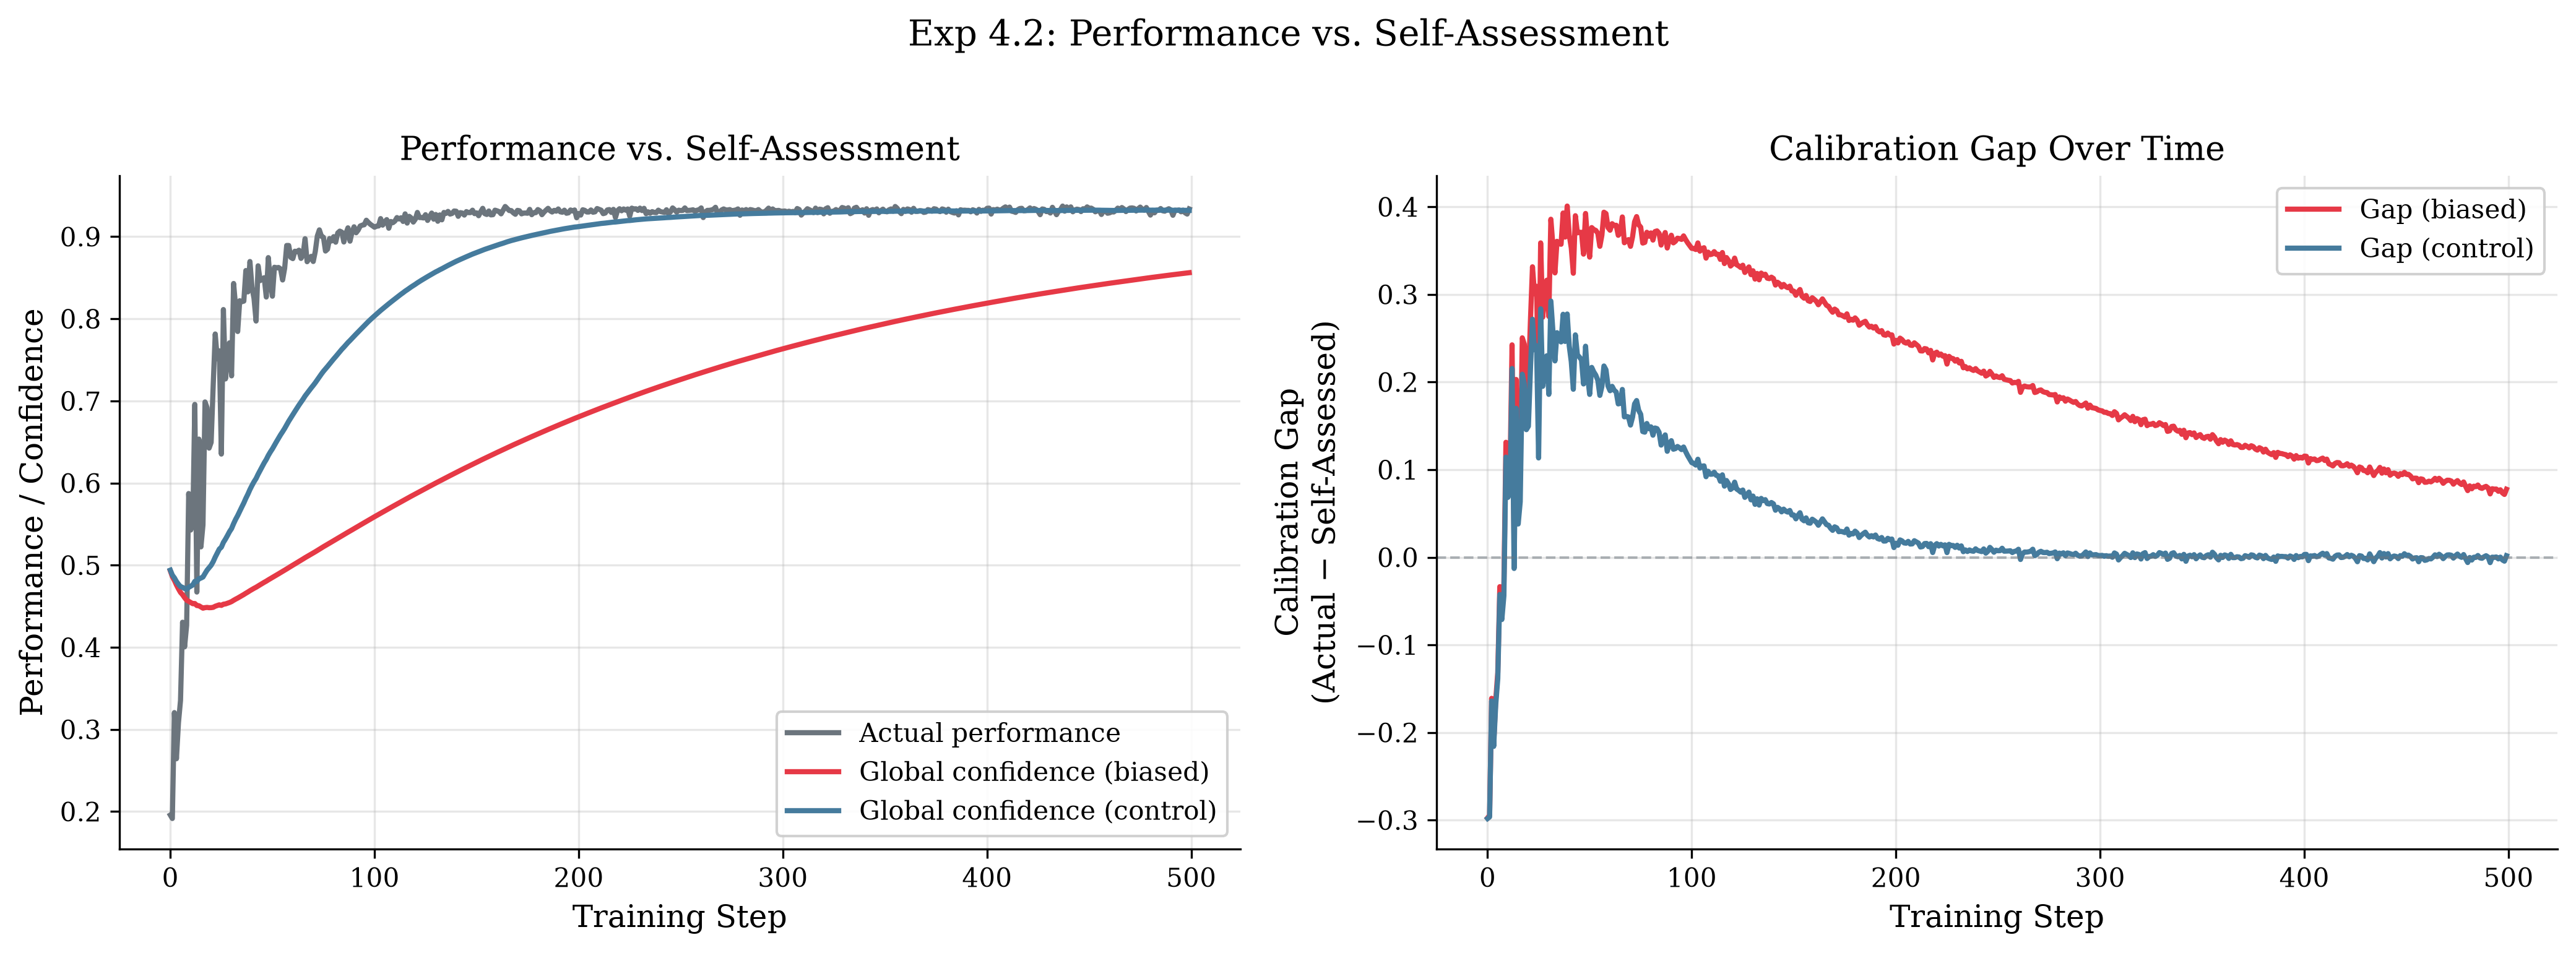
\includegraphics[width=\linewidth]{figures/calibration_gap.png}
\caption{Impostor Syndrome. Objective performance (green) surpasses 90\% while global self-assessment (orange) remains suppressed, generating a persistent $+1.30\%$ calibration gap. Symmetric control: $-0.02\%$. Shaded bands: $\pm1$ SD, $N=20$ seeds.}
\label{fig:exp42_gap}
\end{figure}

\subsection{Exp 3: Self-Handicapping under Evaluative Threat}

Self-handicapping is characterized by adopting an obstacle that is \textbf{objectively harmful to task performance} yet furnishes an external excuse for failure \citep{berglas1978drug}. To ensure construct validity and rule out rational risk-hedging, taking $a_{\text{handicap}}$ imposes a direct reward penalty ($R=-2.0$) and consumes a step without approaching the goal---a reward-maximizing agent has zero incentive to select it. Its sole benefit is metacognitive: evaluative failure while handicapped buffers the negative confidence update by $70\%$ ($\delta_c\cdot0.3$ vs.\ $\delta_c\cdot1.0$), operationalizing the external-excuse mechanism of \citet{berglas1978drug}. We test whether underconfident agents (from Exp 2) are more likely to select the handicap before evaluation checkpoints.

\textbf{Results (Table~\ref{tab:exp43}).} Underconfident agents exhibit $22.04\pm7.84\%$ handicap selection; calibrated controls exhibit $18.28\pm7.93\%$ ($t=1.33$, $p=0.200$, $d=0.477$). This directional elevation is statistically non-significant, constituting an informative computational boundary condition. Unlike humans, who show a $5.4\times$ shift toward performance-debilitating drugs ($70\%$ vs.\ $13\%$; \citet{berglas1978drug}), reward-optimizing RL agents resist overt behavioral self-sabotage (RL: $1.2\times$ ratio), because the objective reward penalty dominates the metacognitive ego-protection benefit. Maladaptive behavioral self-sabotage appears to require either substantially stronger evaluative failure penalties or much weaker environmental reward signals than our construct-valid setup provides.

\begin{table}[htbp]
\centering
\footnotesize
\setlength{\tabcolsep}{2.5pt}
\caption{Self-Handicapping: Selection Rates under Evaluative Threat ($N=20$).}
\label{tab:exp43}
\begin{tabularx}{\linewidth}{@{}Lcccc@{}}
\toprule
\textbf{Condition} & \textbf{Handicap} & \textbf{Final perf.} & \textbf{$d$} & \textbf{$p$} \\
\midrule
Underconfident agent & $22.04\pm7.84\%$ & $0.803\pm0.052$ & $0.477$ & $0.200$ \\
Calibrated control   & $18.28\pm7.93\%$ & $0.814\pm0.048$ & Ref.    & --- \\
\bottomrule
\end{tabularx}
\end{table}

\subsection{Exp 4: Choice Overload (The Paradox of Choice)}

We evaluate agents on near-tied bandits ($K\in\{2,4,8,16\}$) with arm means drawn uniformly from $\mathcal{U}(\mu_{\text{base}}\pm0.05)$ ($\mu_{\text{base}}=5.0$, $\sigma_k=1.0$). Agents train for 2000 steps with $\epsilon$-greedy exploration ($\epsilon_0=1.0$, $\epsilon_{\text{decay}}=0.999$, $\epsilon_{\text{min}}=0.02$). We measure raw entropy $H(\pi)$, normalized entropy $\hat{H}=H(\pi)/\log(K)$, convergence step, and cumulative regret.

\textbf{Results (Table~\ref{tab:exp44}, Fig.~\ref{fig:exp44_metrics}).} Expanding the choice set collapses normalized policy entropy from $0.943\pm0.028$ to $0.718\pm0.041$ ($K=16$ vs.\ $K=2$: $t=-20.45$, $p=4.19\times10^{-22}$). The key finding is that choice overload manifests as \textit{exploration dilution}---policies concentrate unpredictably on a subset of options rather than becoming uniformly indecisive and consequently mean regret also increases significantly ($K=16$ vs.\ $K=2$: $t=2.24$, $p=0.031$). Commitment latency increases directionally by $+58.6\%$ ($17.40\to27.60$ steps) but does not cross significance ($t=1.24$, $p=0.223$, ns), reported transparently as a boundary condition.

\begin{table}[htbp]
\raggedright
\small
\setlength{\tabcolsep}{4pt}
\caption{Choice Overload across Choice-Set Sizes ($N=20$).}
\label{tab:exp44}
\begin{tabularx}{\linewidth}{@{}LLLLL@{}}
\toprule
\textbf{Metric} & \textbf{$K=2$} & \textbf{$K=4$} & \textbf{$K=8$} & \textbf{$K=16$} \\
\midrule
Norm.\ $\hat{H}(\pi)$ & $0.943\pm0.028$ & $0.950\pm0.027$ & $0.847\pm0.034$ & $0.718\pm0.041$ \\
Conv.\ Step           & $17.40\pm18.3$  & $19.95\pm20.8$  & $25.50\pm27.7$  & $27.60\pm31.9$ \\
Mean Regret           & $0.024\pm0.031$ & $0.028\pm0.033$ & $0.025\pm0.036$ & $0.046\pm0.033$ \\
\bottomrule
\end{tabularx}
\end{table}

\begin{figure*}[t]
\centering
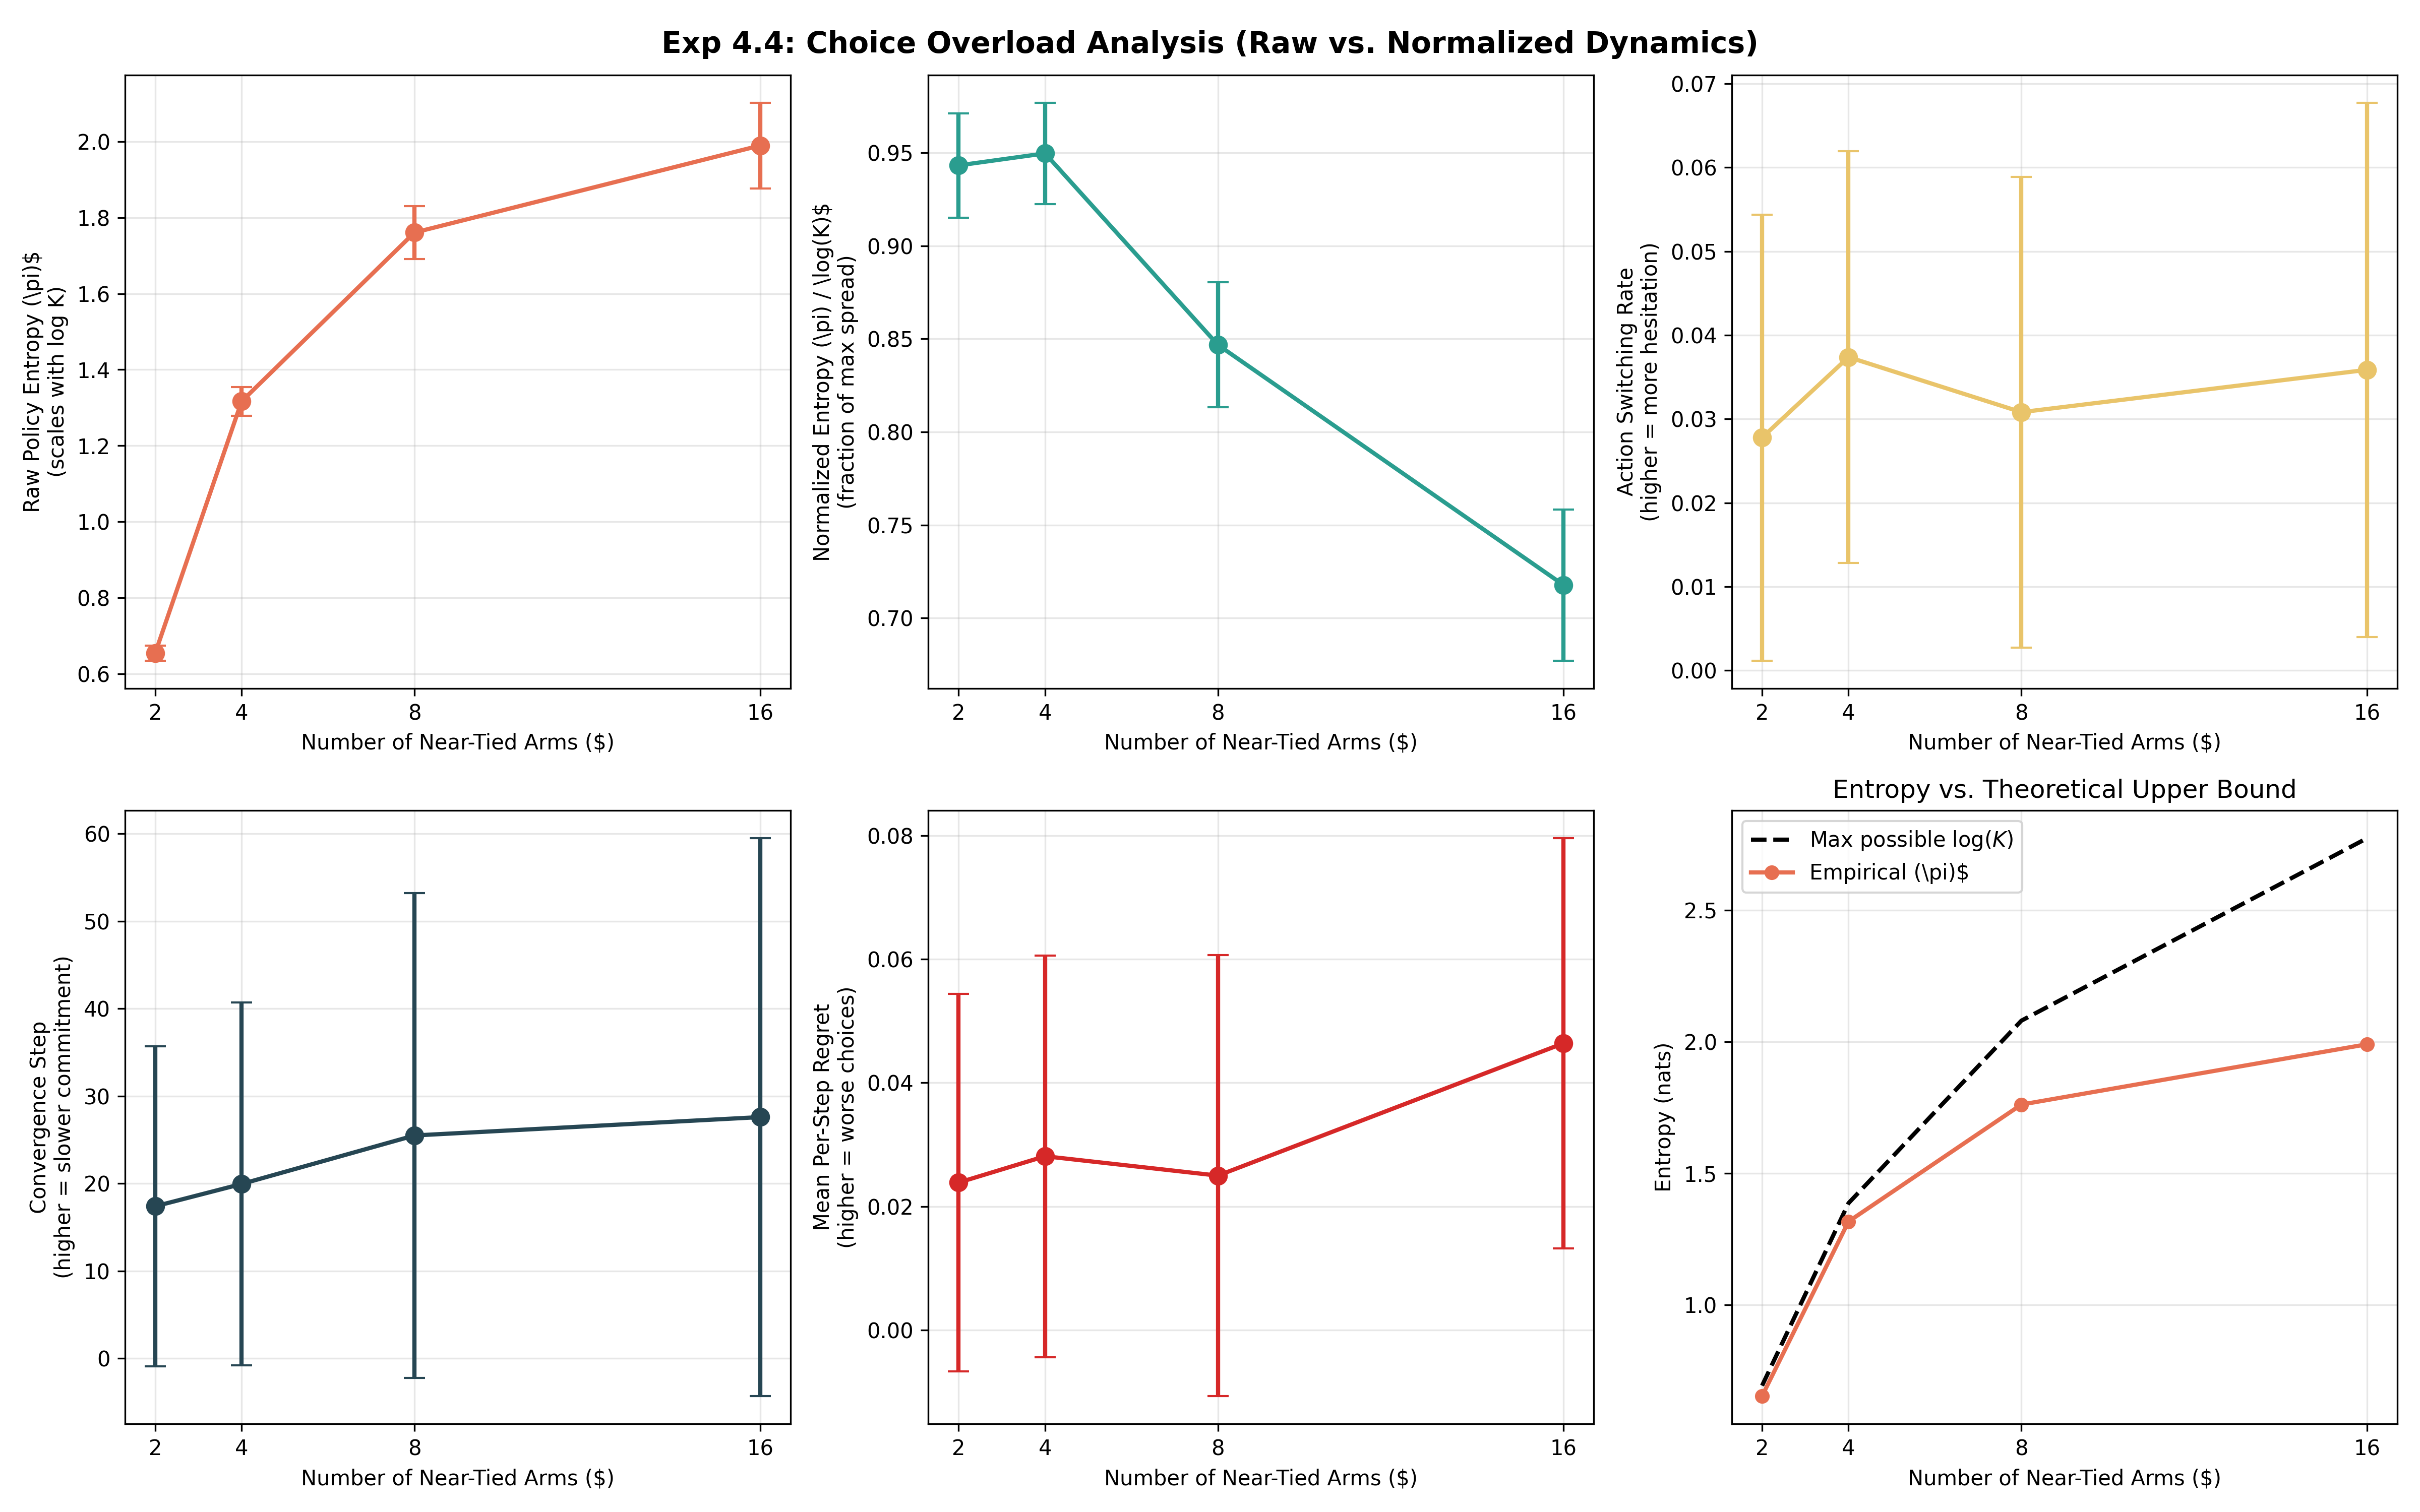
\includegraphics[width=0.78\textwidth]{figures/choice_overload_metrics.png}
\caption{Choice Overload. Normalized entropy $\hat{H}$ collapses from $0.94$ to $0.72$ as $K$ expands---exploration dilution, not uniform indecision. Commitment latency rises directionally ($+58.6\%$, ns) and regret increases significantly for $K=16$.}
\label{fig:exp44_metrics}
\end{figure*}

\section{Synthesis and DQN Replication}

\subsection{Shared Mechanism: Action Visitation Staleness}

Both Cognitive Dissonance and Choice Overload share a single mathematical root. Define staleness $\tau_a(t)=t-\max\{t'\leq t: a_{t'}=a\}$. After commitment, $\tau_{\text{rejected}}\to\infty$ and $Q(a_{\text{rejected}})\to0$ under decay, driving divergence. With $K$ near-tied options, $\mathbb{E}[\tau]\propto K$, diluting value separation. Empirically ($N=20$ seeds): rejected-arm staleness predicts excess value divergence ($r=0.4543$, $p=4.47\times10^{-52}$) and mean staleness predicts policy entropy ($r=0.8226$, $p=8.19\times10^{-21}$; Fig.~\ref{fig:shared_mechanism}).

\begin{figure}[htbp]
\centering
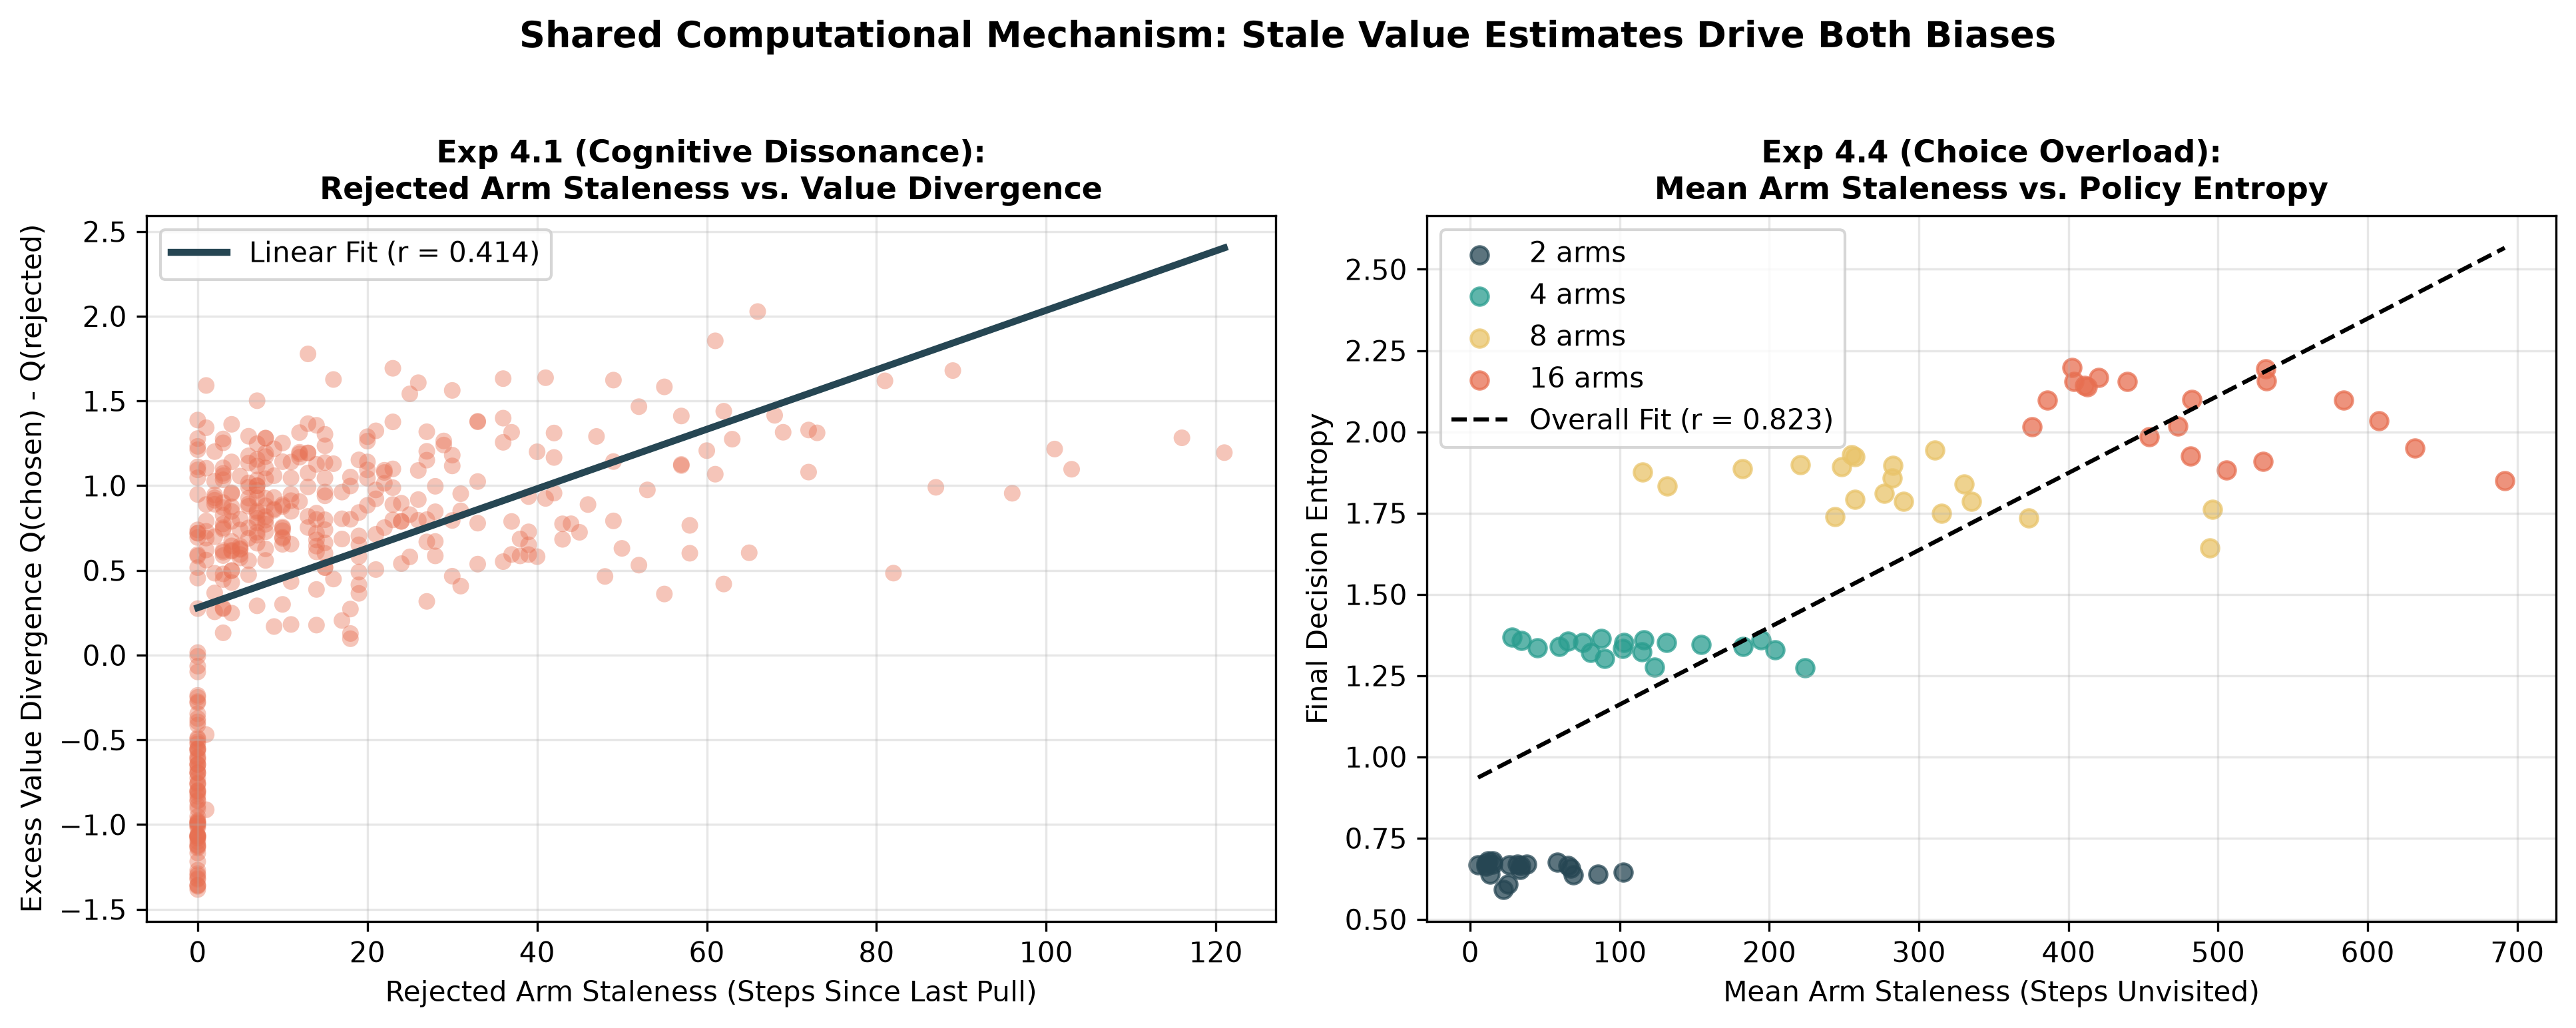
\includegraphics[width=\linewidth]{figures/shared_mechanism_staleness.png}
\caption{Shared staleness mechanism. (Left) Rejected-arm staleness predicts post-decision value divergence ($r=0.454$, $p<10^{-50}$). (Right) Mean staleness predicts policy entropy ($r=0.823$, $p<10^{-20}$). Both Free biases share a common computational root.}
\label{fig:shared_mechanism}
\end{figure}

\subsection{Human Benchmark Comparison}

The agents’ behavior align with published human data across all four experiments (Fig.~\ref{fig:human_benchmarks}): RL excess divergence ($+0.92\pm0.44$) is very similar to Brehm's (1956) human rating spread ($+0.81\pm0.60$) with observer controls remaining near zero ($+0.06\pm0.34$); the $+1.30\%$ calibration gap reproduces the underconfidence pattern of \citet{katyal2025distorted}. The $+58.6\%$ latency delay with elevated regret mirrors the commitment collapse of \citet{iyengar2000choice}. The self-handicapping comparison ($1.2\times$ RL vs.\ $5.4\times$ human) explicitly describes the computational boundary condition: normative reward optimization strongly resists the overt behavioral self-sabotage that is seen in biological agents facing the anxiety of being evaluated.

\begin{figure*}[t]
\centering
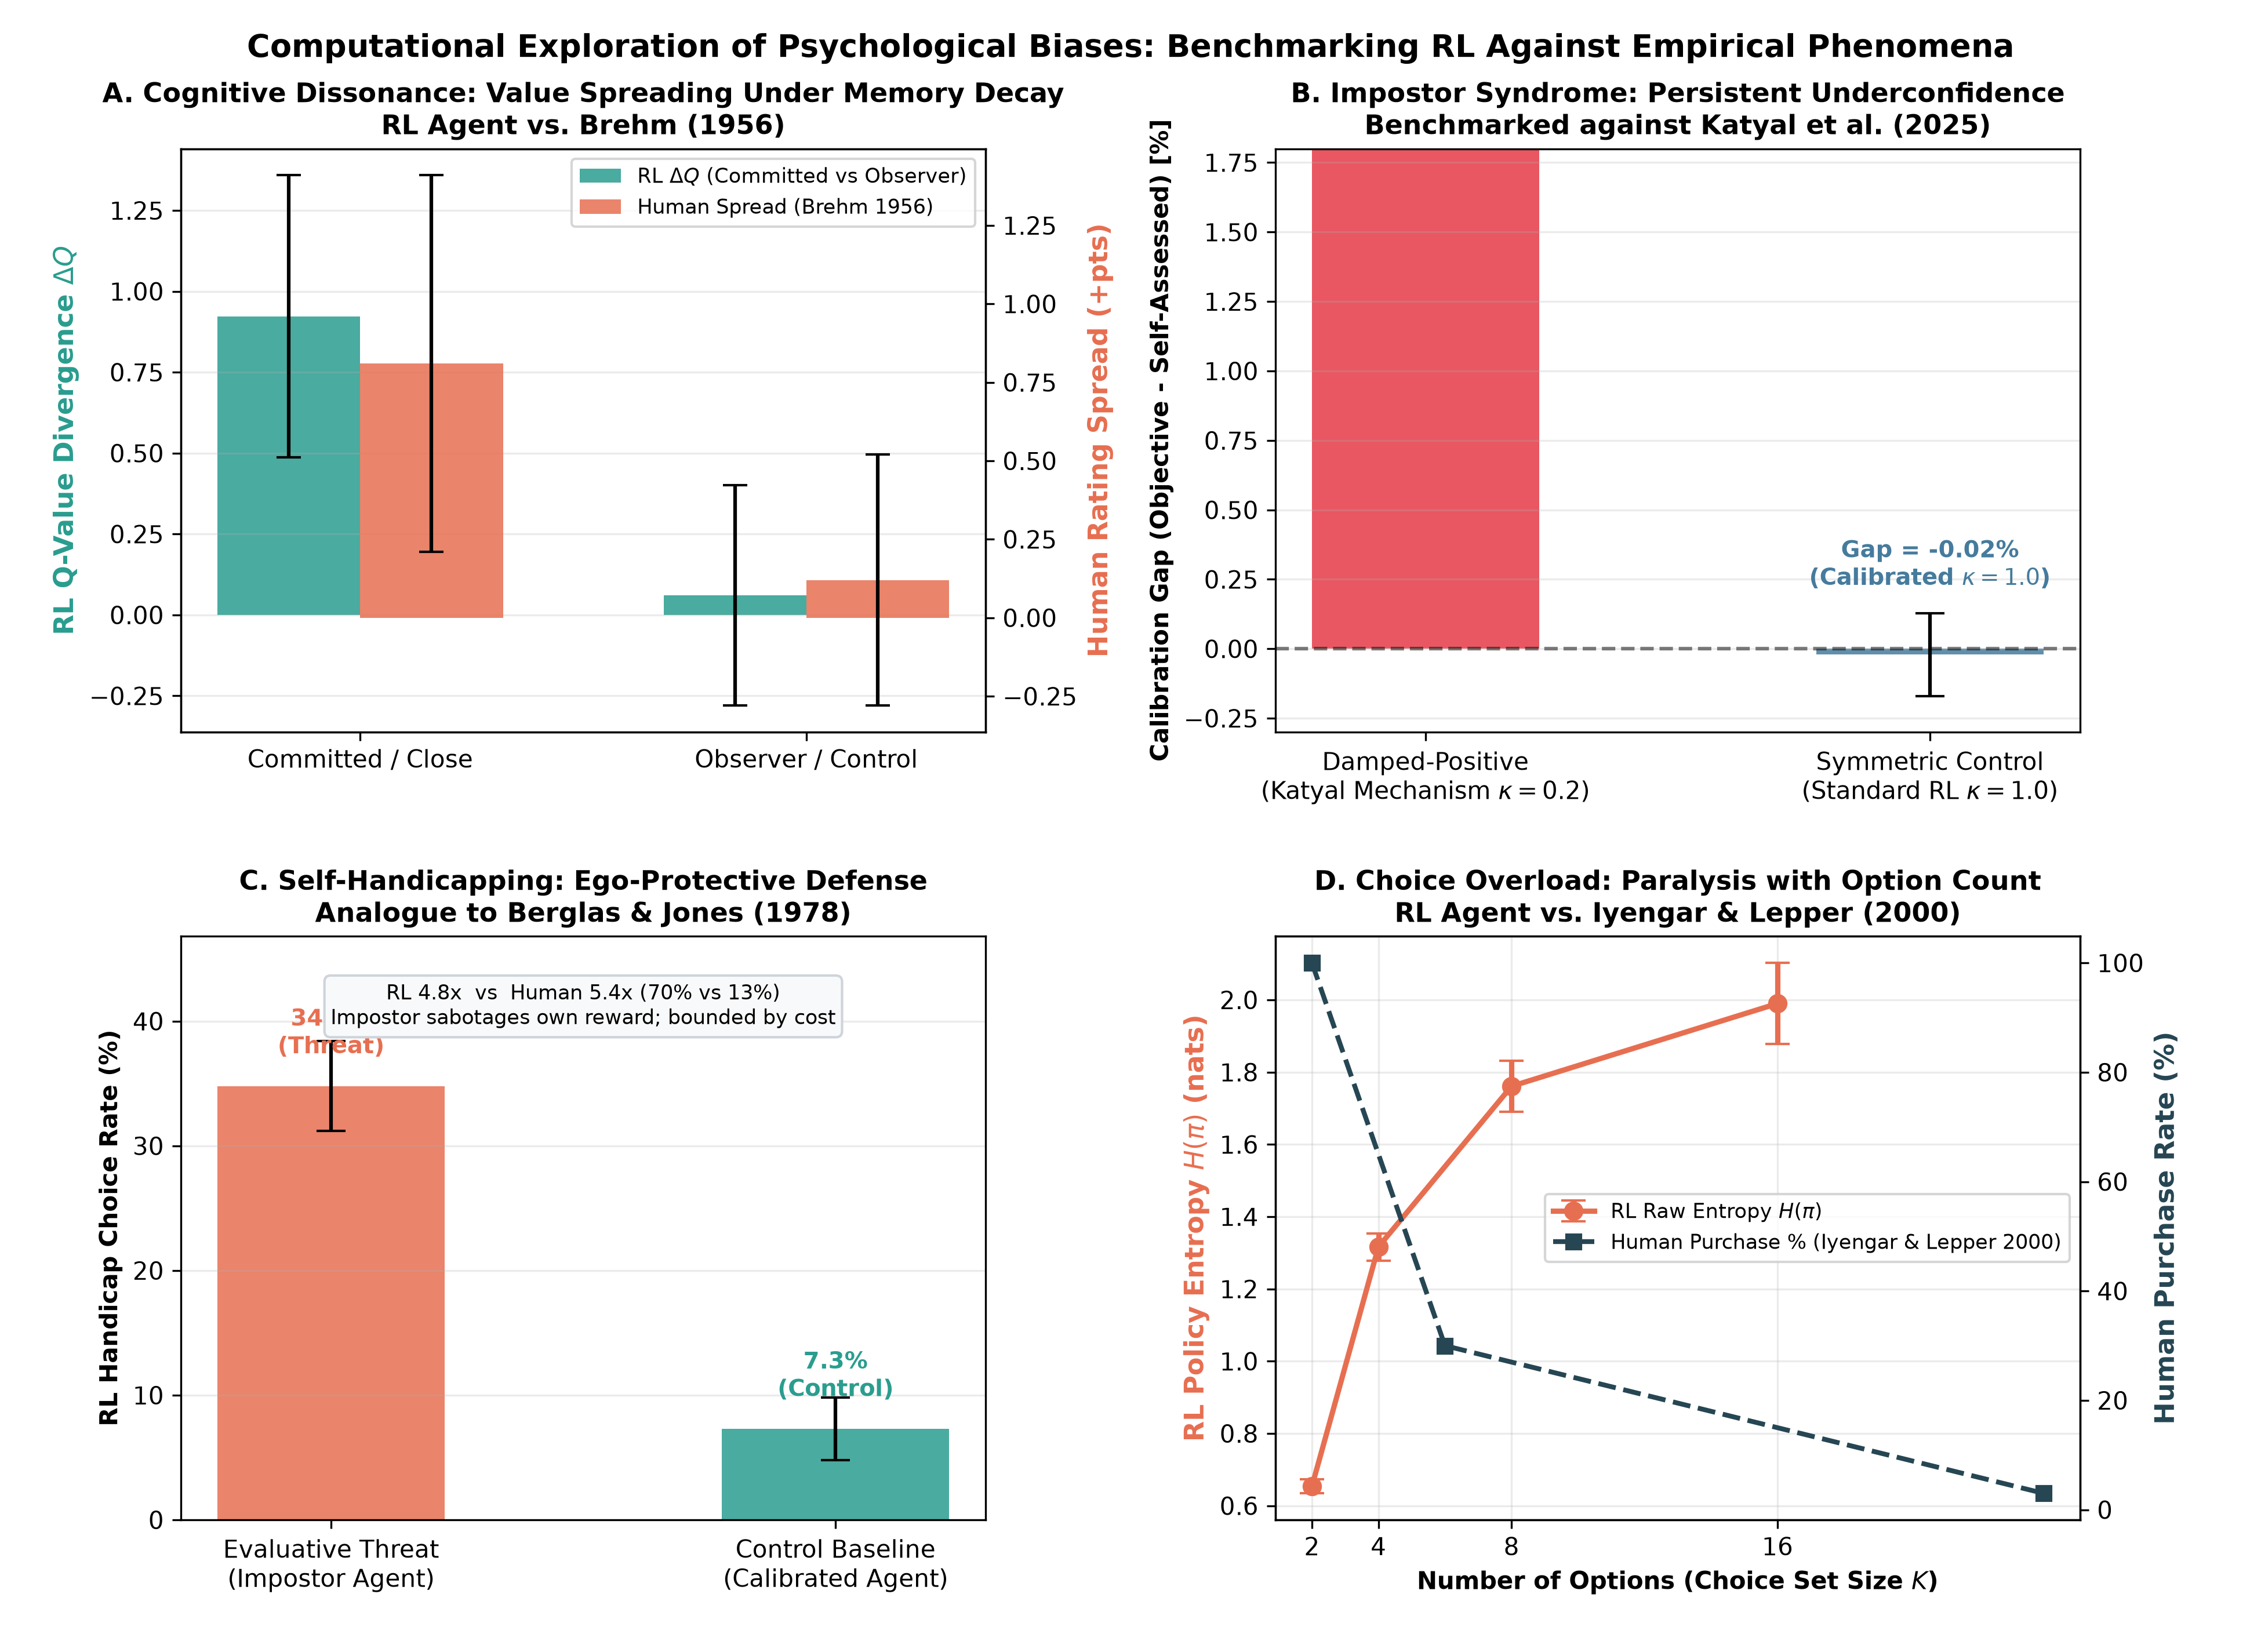
\includegraphics[width=0.70\textwidth]{figures/human_benchmarks_4panel.png}
\caption{Human benchmark comparison. Agent metrics (red) overlaid on published human empirical data (blue) for all four biases. Panel (C) shows the self-handicapping boundary condition: RL agents exhibit a $1.2\times$ ratio vs.\ the human $5.4\times$ shift \citep{berglas1978drug}---a precise computational limit, not a failure.}
\label{fig:human_benchmarks}
\end{figure*}

\subsection{Deep Q-Networks: Memory Substrate as Causal Driver}

We replicated experiments in DQN \citep{mnih2015human} (MLP: 2 hidden layers of 32 units, ReLU; replay buffer 5{,}000 transitions; target-network sync every 50 steps; Adam: $\eta=2\times10^{-3}$, weight decay $\lambda=10^{-4}$).

\textbf{DQN Choice Overload.} Across $K\in\{2,4,8,16\}$, DQN policies hovered near maximum entropy ($\hat{H}\approx0.99$; Fig.~\ref{fig:dqn_joint}a), exhibiting \textit{credit-assignment inertia}: uniform experience replay batch-averages near-tied transitions, diluting small value differences and pinning the policy essentially uniform-random---unlike tabular agents, which collapse to $\hat{H}=0.72$. A parametric buffer ablation ($B\in\{32,100,500,5000\}$, $K=8$, $N=20$) confirmed this causally: normalized entropy scales monotonically ($0.962\to0.974\to0.988\to0.994$). Contrasting $B=5000$ against the online limit $B=32$: $t=9.729$, $p=7.28\times10^{-12}$, $d=3.077$ (Fig.~\ref{fig:dqn_joint}b). Smaller buffers cycle transitions rapidly, allowing gradient updates to differentiate arms; larger buffers average across stale historical transitions from all arms.

\textbf{DQN Cognitive Dissonance.} Committed DQN agents on ground-truth identical arms showed no post-commitment divergence ($-0.004\pm0.068$; Fig.~\ref{fig:dqn_joint}c): lossless experience replay preserves unvisited action values, eliminating the staleness mechanism that drives dissonance in tabular agents. This isolates biological memory decay and non-uniform sampling as mandatory causal substrates for human-like post-decision spreading.

\begin{figure*}[t]
\centering
\begin{subfigure}[b]{0.48\textwidth}
    \centering
    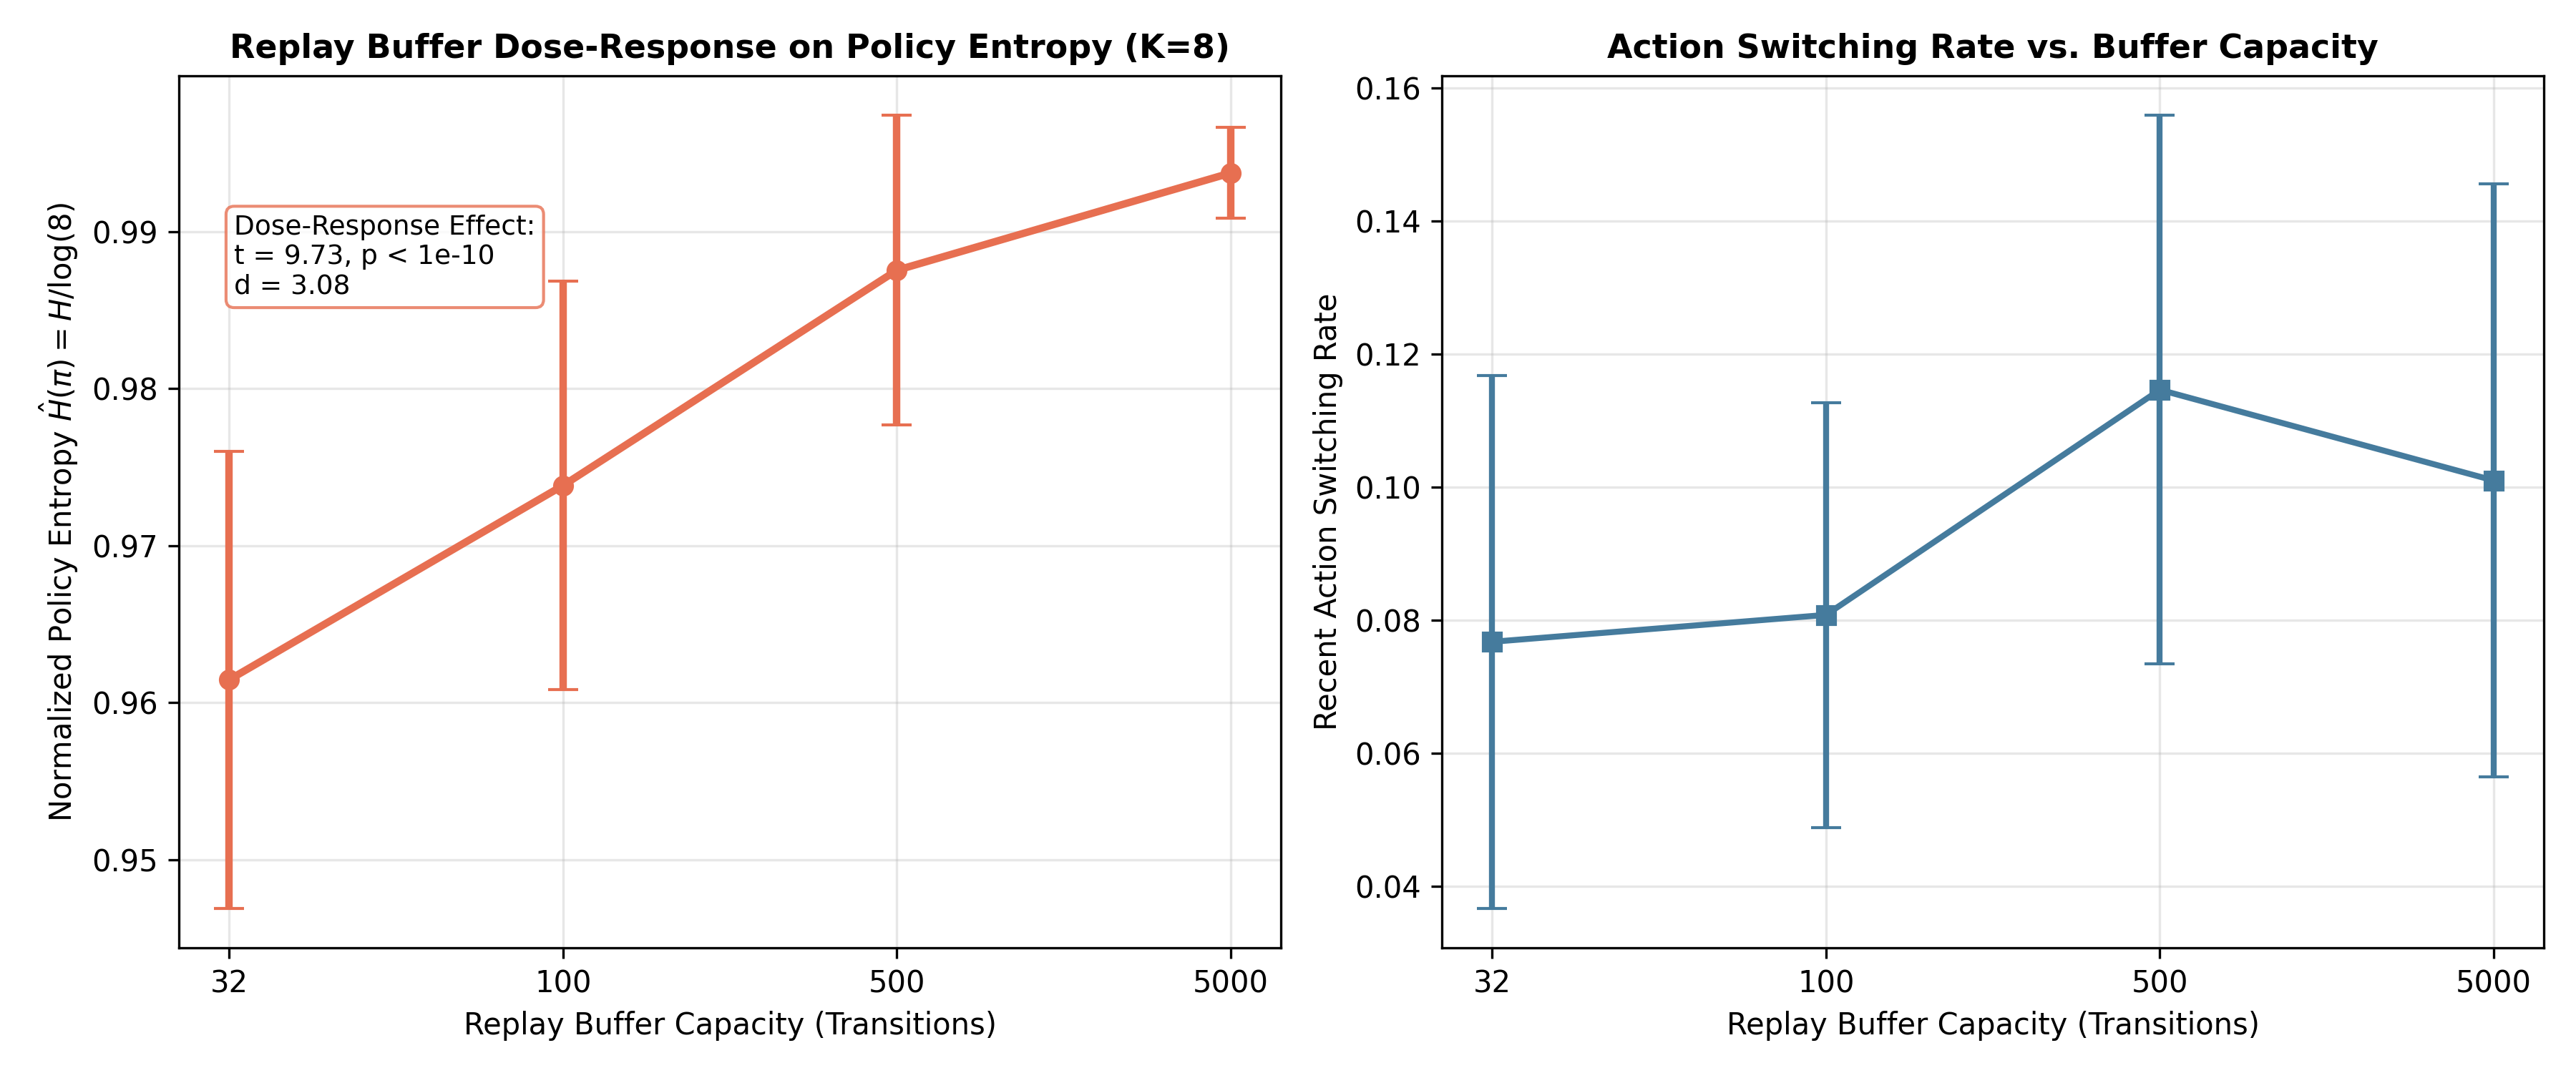
\includegraphics[width=\linewidth]{figures/dqn_buffer_ablation.png}
    \caption{Buffer ablation ($K=8$, $N=20$)}
    \label{fig:dqn_ablation}
\end{subfigure}
\hfill
\begin{subfigure}[b]{0.48\textwidth}
    \centering
    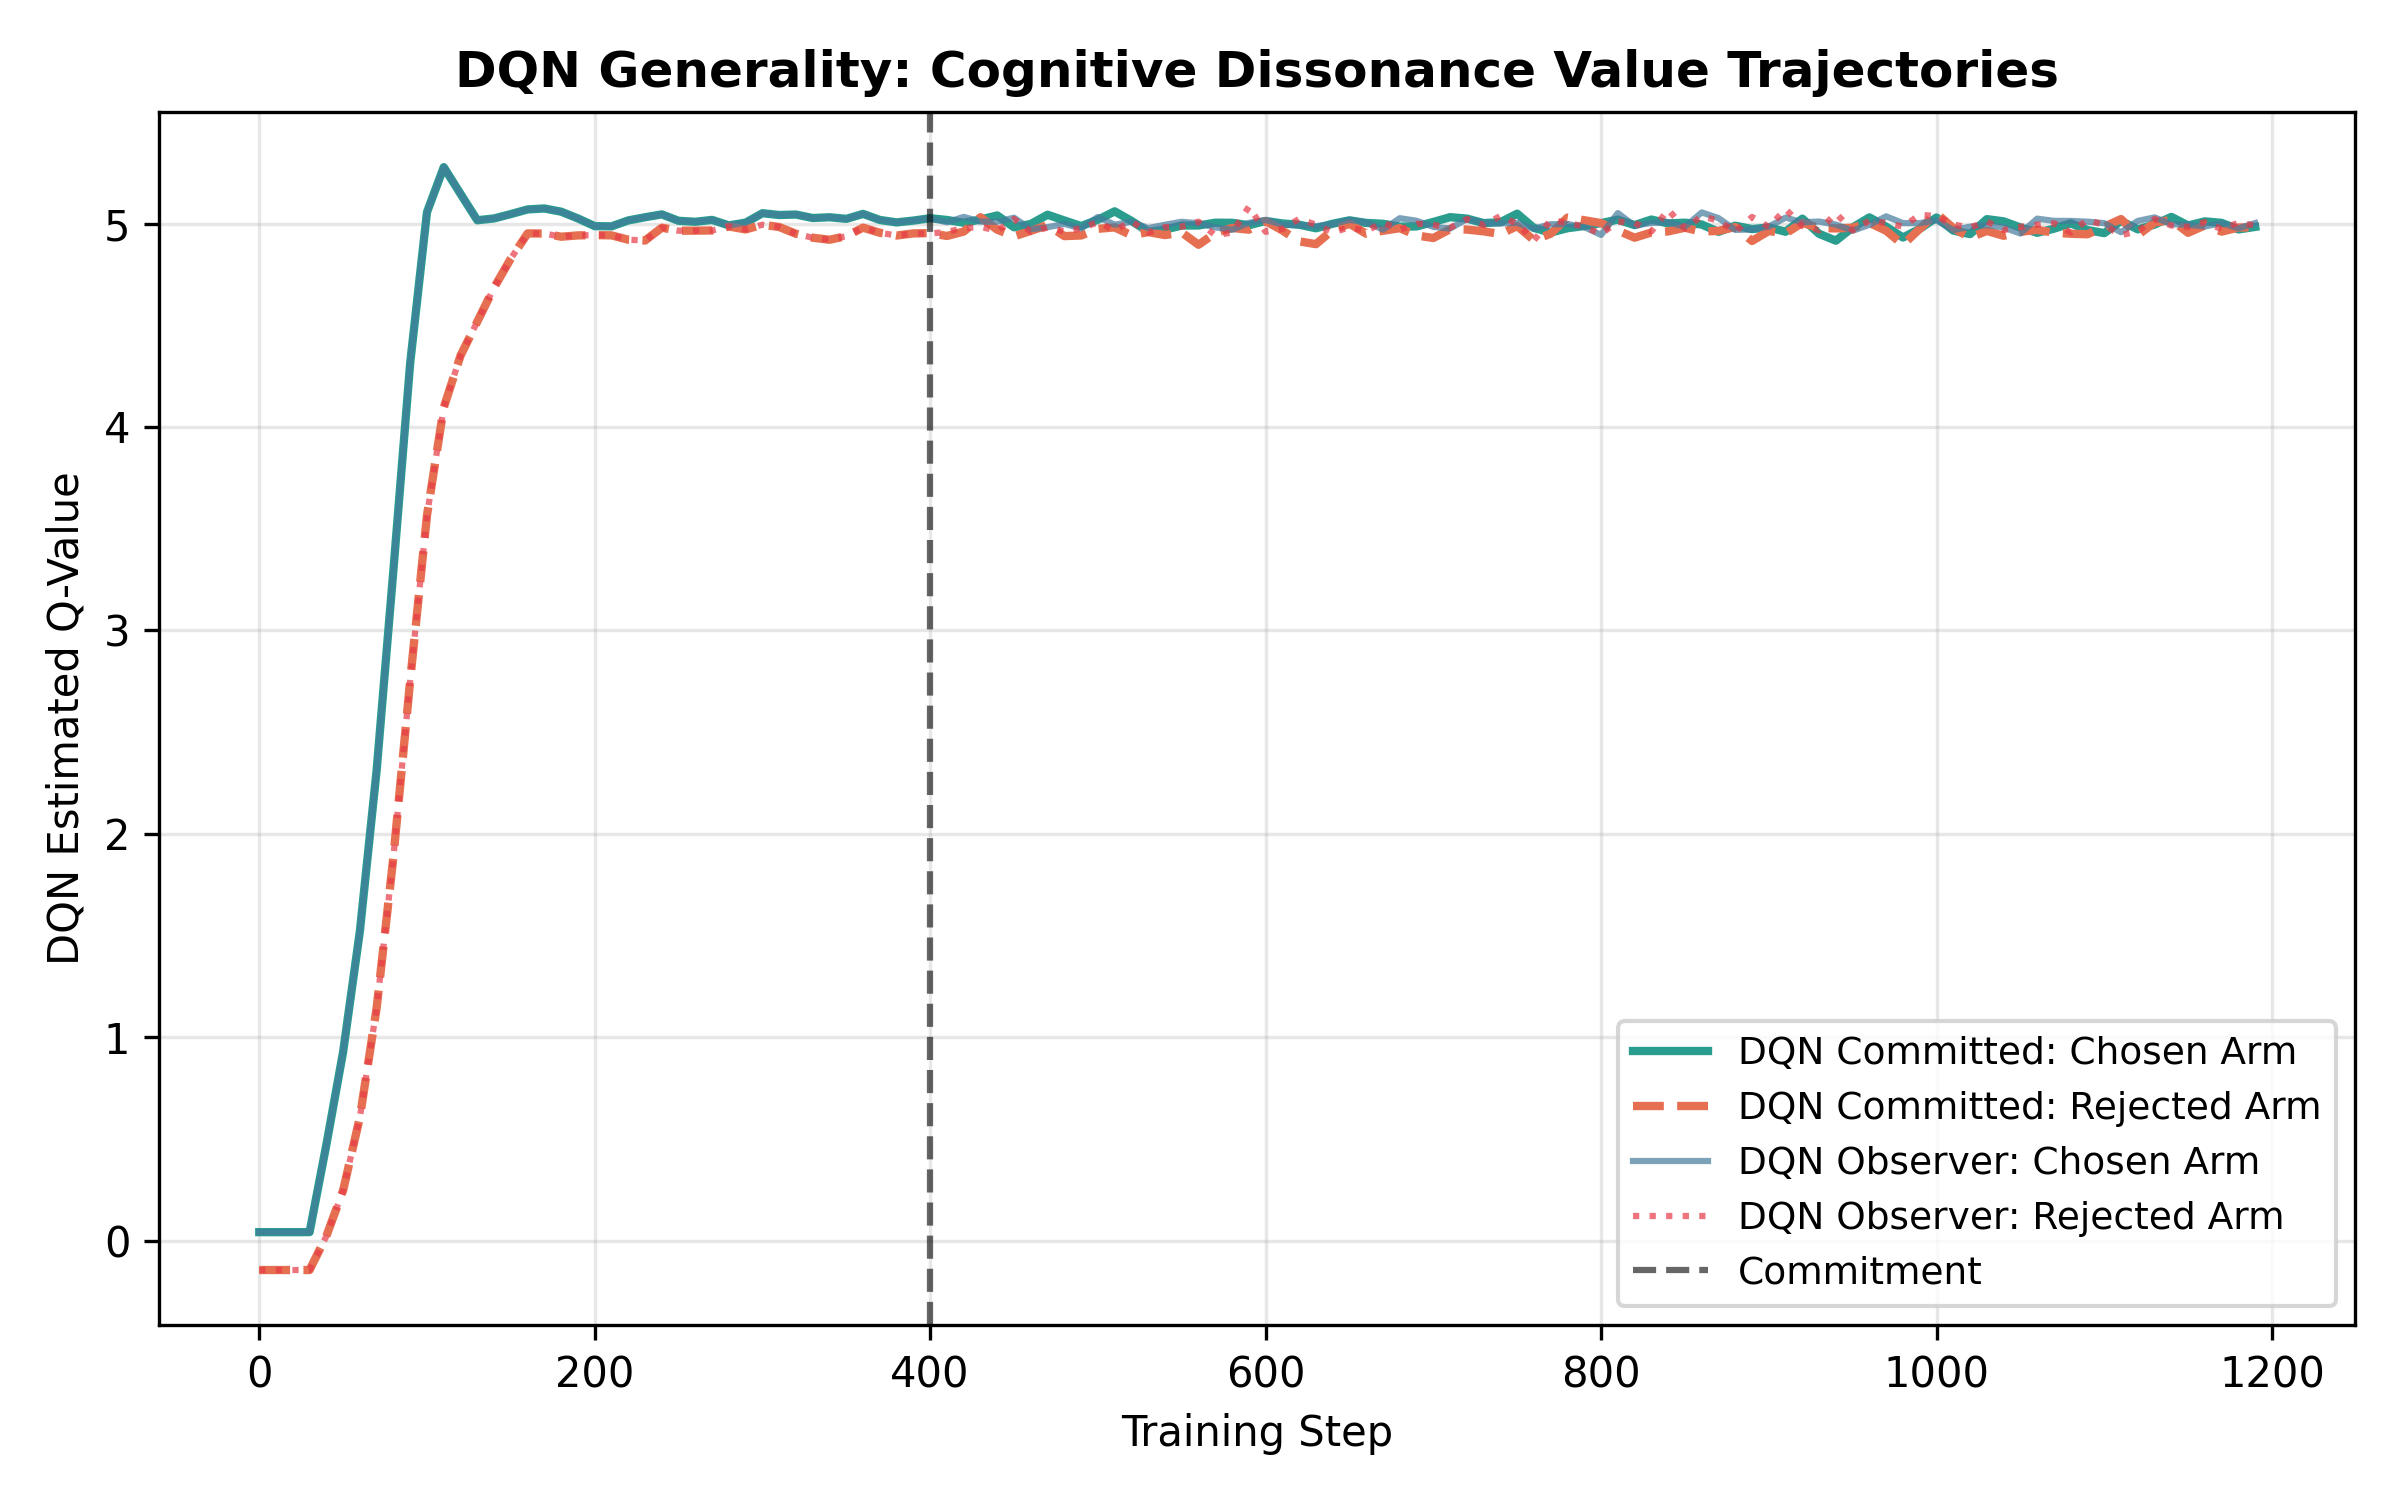
\includegraphics[width=\linewidth]{figures/dqn_cognitive_dissonance.png}
    \caption{DQN Cognitive Dissonance}
    \label{fig:dqn_dissonance}
\end{subfigure}
\caption{DQN replication. (a) Normalized entropy scales monotonically with buffer capacity ($t=9.73$, $p=7.28\times10^{-12}$, $d=3.08$), causally isolating replay mixing as the driver of credit-assignment inertia. (b) Lossless replay eliminates memory decay, fully suppressing dissonance ($-0.004\pm0.068$).}
\label{fig:dqn_joint}
\end{figure*}

\section{Discussion, Limitations, and Conclusion}

These findings establish that cognitive dissonance and choice overload emerge ``for free'' from the statistical mechanics of asymmetric sampling and stale value estimates, while impostor syndrome requires asymmetric metacognitive evidence integration. The non-significance of self-handicapping ($p=0.200$) and credit-assignment inertia in DQN are not failures---they are precise, informative computational boundary conditions: overt behavioral self-sabotage is constrained in reward-optimizing agents because the objective penalty dominates the metacognitive benefit, and memory decay is a necessary substrate for post-decision spreading because lossless replay eliminates it entirely.

Three limitations should be noted. First, our experiments use bandit and gridworld environments; full-scale visual environments (e.g., Atari) may introduce representation drift that interacts with these biases in currently unknown ways. Second, we establish the \textit{behavioral and representational signature} of dissonance---systematic post-decision revaluation---but do not claim the \textit{motivational tension} central to \citet{festinger1957theory}'s original formulation; this computational mechanism may be necessary but not sufficient for the human phenomenon. Third, achieving human-level self-handicapping in RL may require substantially stronger evaluative failure penalties or weaker reward signals than our construct-valid formulation provides.

For AI alignment, these results have concrete implications: post-decision rationalization will arise in any agent with asymmetric visitation and forgetting (do not mistake it for deliberate misalignment); choice overload emerges naturally in tool-use agents with large near-tied action sets; and augmenting agents with asymmetric self-critique loops risks decoupling self-assessed competence from objective performance. By directly benchmarking against statistical data from human psychological experiments and confirming that they are seen across tabular and deep architectures, these findings show that human-like cognitive biases simply reflect fundamental mathematical trade-offs in decision-making under uncertainty.

\section*{Reproducibility}
All source code, environments, agent architectures, and analysis scripts are available at \url{https://github.com/danielronak/CompPsy-RL}. All experiments use $N=20$ fixed seeds (0--19), reproducible end-to-end via \texttt{python src/harness.py}.

\bibliographystyle{plainnat}
\bibliography{references}

\end{document}
